Sběrnice MTBbus vznikla v roce 2000 \cite{mtb:web}, kdy se hledal vhodný systém
pro programovatelné počítačové řízení modelové železnice v Klubu modelářů
železnic Brno I (\gls{kmz}), jehož je autor této práce členem.
\textit{Digital Command Control} (\gls{dcc}), dnes nejšířeji používaný
mezinárodně standardizovaný systém pro digitální řízení modelové železnice
\cite{dcc_intro:web} tehdy ještě nebyl v českých končinách zaužívaný. Navíc
přirozeně vyvstal požadavek na minimalizaci nákladů a maximalizaci nezávislosti
na konkrétních komerčních produktech. Skupina nadšenců tedy vytvořila systém
\gls{mtb}, který se pro řízení modelových kolejišť ve výše zmíněném klubu
používá doteď \cite{kmz_rizeni:web}.

\section{Popis sběrnice \gls{mtbbus}} \label{sec:mtbbus}

Každé kolejiště má svou vlasní sběrnici \gls{mtbbus}, ke které je připojený
právě jeden \textit{MTB-USB} modul a až 255 \gls{mtb} modulů. \textit{MTB-USB}
modul řídí provoz na celé sběrnici, ostatní \gls{mtb} moduly pouze odpovídají
na příkazy \textit{MTB-USB} modulu. Říkáme, že sběrnice je \textit{single
master, multiple slaves} \ref{fig:mtbbus-topology}.

Každý \gls{mtb} modul má:

\begin{compactenum}
\item 8bitovou adresu, která se konfiguruje jumpery přímo na modulu,
\item konfiguraci (typ vstupů/výstupů, rychlost sběrnice, ...),
\item vstupy (stav vstupů),
\item výstupy (stav výstupů).
\end{compactenum}


\begin{figure}[ht]
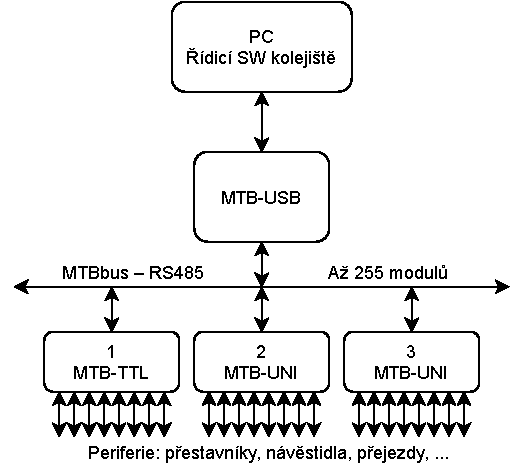
\includegraphics[width=0.7\textwidth]{data/mtb-topology.pdf}
\caption{Topologie systému \gls{mtb}.}
\label{fig:mtbbus-topology}
\end{figure}

\begin{table}[h]
	\begin{tabularx}{\textwidth}{XX}
		\toprule
		Typ přenosu & RS485, formát dat UART \\
		Komunikační rychlost & 38400~Bd, 57600~Bd, 115200~Bd \\
		Maximální počet modulů & 255 \\
		Počet datových bitů & 9 \\
		Stop bit & 1 \\
		Parita & žádná \\
		Maximální délka vedení & 100 m \\
		\bottomrule
	\end{tabularx}
	\caption{Základní parametry sběrnice \gls{mtbbus}}
	\label{tab:mtbbus-params}
\end{table}

Současná implementace sběrnice je založena na elektrickém standardu RS485.
Sběrnice RS485 je dvouvodičová (\textit{R+, R-, GND}) poloduplexní
diferenciální komunikační sběrnice vyvinutá s důrazem na odolnost vůči
externímu rušení. Je vhodná pro přenos dat na větší vzdálenosti, řádově desítky
až stovky metrů. Pro dosažení nejlepších elektrických vlastností by sběrnice
měla být lineární. Sběrnice je na obou koncích termínována rezistorem
\textit{200 R} a pull-up a pull-down rezistory pro držení definované úrovně
signálu.

Sběrnice RS485 je velice snadno implementovatelná do prakticky všech
mikrokontrolérů – stačí rozhraní UART, jeden pin pro řízení směru komunikace
a driver k RS485.

Na sběrnici mohou být \gls{mtb} moduly různého typu:

\begin{itemize}
\item \textbf{MTB-UNI}

	MTB-UNI (\textit{univerzální}) je nejpoužívanější typ modulu. Obsahuje 16
	digitálních vstupů a 16 digitálních výstupů. Na výstupech 0–7 umožňuje kódovat
	návěst protokolem S-COM \cite{}, což umožňuje připojení až 8 návěstidel
	k jednomu modulu MTB-UNI. Modul dále umožňuje připojení IR čidel na vstupy,
	což jsou rozšířená bodová čidla detekující průjezd vlaku. Pro použití IR
	čidel je třeba speciálním způsobem budit vysílací IR diodu, což si žádá podporu
	ve speciálním hardwaru na desce. Výstupu modulu jsou v režimu otevřeného
	kolektoru a umožňují maximální zátěž až 0.5~A / 8 výstupů.

\item \textbf{MTB-TTL}

	MTB-TTL je zjednodušený modul MTB-UNI. Oproti modulu MTB-UNI neobsahuje
	podporu IR čidel a výstupy má v režimu TTL. Od tohoto typu modulu se v
	současnosti ustupuje, neboť TTL výstupy nejsou vhodné pro spínání vyšších
	napětí (např. 12~V) a proto, že v případě neaktivního výstupu (+5~V –
	inverzní logika) aktivně napájí výstupní port, což způsobuje nechtěné chování,
	pokud je ne výstupním portu záměrně vypnutá periferie. V krajním případě může
	dojít až k přetížení TTL výstupu a jeho zničení. Na všechny nasazené moduly
	typu MTB-TTL byly postupně instalovány dodatečné obvody s otevřenými
	kolektory na výstupy.

\item \textbf{MTB-REG}

	MTB-REG je modul umožňující generovat analogový výkonový výstup. Modul se
	připojí ke kolejím a řídí rychlost a směr lokomotiv v řízeném úseku.

	Tento způsob řízení jízdy (tzv. \textit{analogový}) je dnes již překonaný.
	V současnosti se pro řízení jízdy lokomotiv na kolejišti používá tzv. systém
	\textit{Digital Command Control} \cite{dcc}, kde každá lokomtiva a mnohdy
	i vagóny v sobě mají mikroprocesor a celý systém je řízen digitálně.

	Modul MTB-REG je tedy již překonaným modulem a autor jej uvádí spíš pro
	úplnost popisu systému \gls{mtb}.

\item \textbf{MTB-POT}

	Modul MTB-POT obsahuje 4 analogové vstupy a 4 digitální vstupy. Jeho
	původním záměrem bylo, že se připojí k potenciometru v pultu obsluhy
	kolejiště, kterým obsluha reguluje jízdu vlaku. Po sběrnici přepošle data
	modulu \textit{MTB-REG} a tím dojde ke kýžené jízdě vlaku. Tento způsob
	řízení jízdy na kolejištích se již nepoužívá, proto i modul \textit{MTB-POT}
	pozbyl svého smyslu.

\end{itemize}

\begin{figure}[ht]
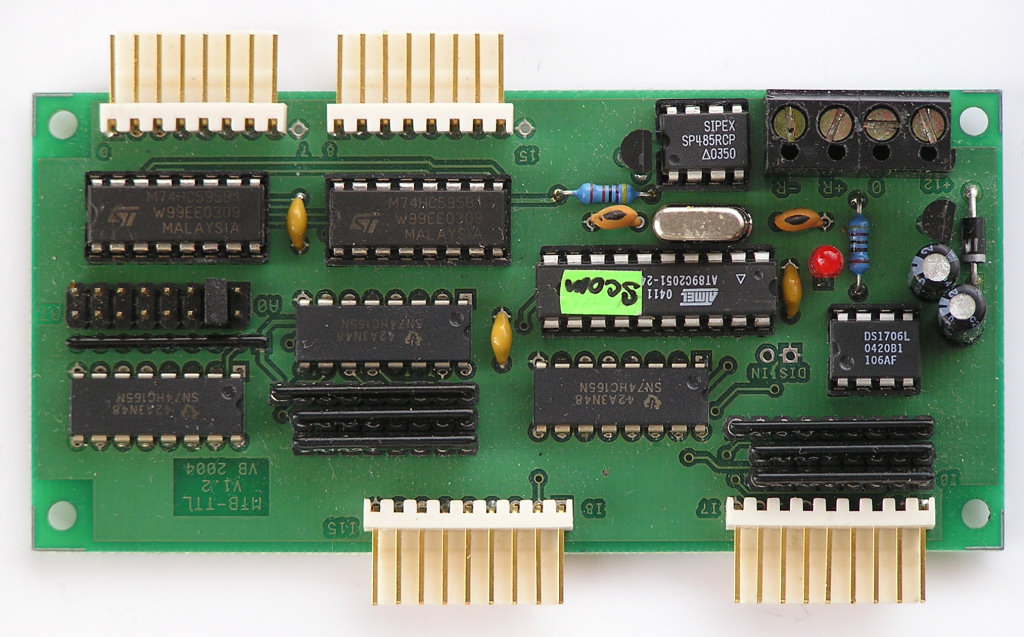
\includegraphics[width=0.7\textwidth]{data/mtbttl_foto.jpg}
\caption{Ukázka modulu MTB-TTL \cite{mtb:web}.}
\label{fig:mtbttl}
\end{figure}

Po sběrnici se komunikuje definovaným protokolem \cite{mtbbus-proto}. Protokol
definuje příkazy pro moduly, odpovědi modulů, časování apod.

Práce se sběrnicí z pohledu aplikace v počítači probíhá následovně:

\begin{compactenum}
\item Připojit se k MTB-USB modulu.
\item Provést sken aktivních modulů sběrnice.
\item Nahrát do všech aktivních modulů konfiguraci.
\item Přečíst stav vstupů.
\item Zahájit provoz – od teď všechny moduly nahlašují změny stavů vstupů.
\item Číst vstupy, nastavovat výstupy.
\item Ukončit komunikaci.
\item Uzavřít spojení s MTB-USB.
\end{compactenum}

\section{IR čidla} \label{sec:uni_ir}

Nyní popíšeme princip fungování IR čidel v kolejišti, protože bude v dalších
kapitolách stěžejní.

IR čidlo je bodový detektor průjezdu vlaku. Do kolejí se vedle sebe umístí
opticky oddělená vysílací dioda a fototranzistor. při průjezdu vlaku dojde k
odrazu signálu od spodku vozu nebo lokomotivy, čímž je detekován průjezd vlaku.
Výhodou je nenápadná instalace mezi pražce, která neruší celkový dojem modelu.

TODO obrázek v kolejích

Pro spolehlivou detekci odrazu od matných černých povrchů podvozků je třeba
budit vysílací diodu vysokým proudem (řádově 200 mA), což vyžaduje použití
diody v impulsním režimu. \textit{MTB-UNI} deska podporuje IR čidla na všech
svých 16 vstupech, diody jsou buzeny tranzistory ve skupinách po 4 diodách.

Aby bylo zajištěno spolehlivé vyhodnocení odraženého signálu, je vstup z
fototranzistoru zapojen na digitální vstup postuvného registru přes kapacitní
vazbu.

Vstupy \textit{MTB-UNI} desky se konfigurují osazením rezistorových lišt nebo
kondenzátorů do běžného nebo režimu nebo do režimu snímání IR čidla. Kromě
toho musí o režimu pinu vědět i procesor, aby adekvátním způsobem zpracovával
vstupní signál.

TODO obrázek kapacitní vazby

\textit{MTB-UNI} desky obsahují podporu IR čidel.

\section{Systém \gls{mtb} v kontextu řízení celého kolejiště} \label{sec:mtb_context}

V \gls{kmz} je aktuálně systém \gls{mtb} nasazen na dvou kolejištích, další
nasazení je na modulovém kolejišti Mendelovy univerzity v Brně, s kterou klub
spolupracuje. Na těch kolejištích je aktuálně nasazeno 99 MTB desek.

Pro zajímavost uveďme, jak systém MTB zapadá do celkové koncepce řízení
kolejiště.

\begin{figure}[ht]
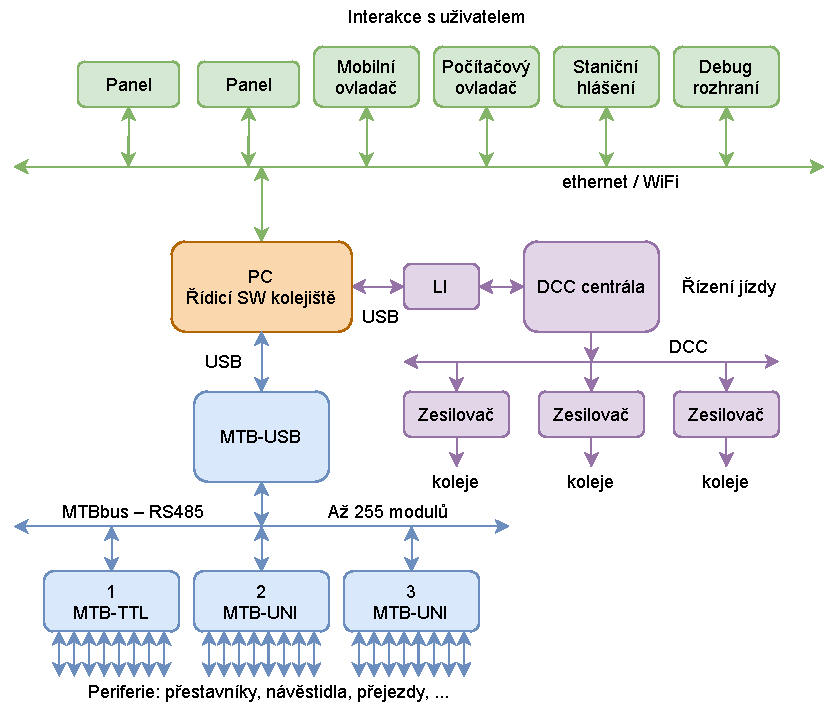
\includegraphics[width=\textwidth]{data/railroad-topology.pdf}
\caption{Schéma komponent řízení kolejiště v \gls{kmz}.}
\label{fig:railroad-topology}
\end{figure}

Autor si rovnou dovolí uvést, že komplikovanější systém řízení modelového
kolejiště snad nemá v Česku a na Slovensku obdobu. Na první pohled je vidět,
že kolejiště je řízeno dvěma různými systémy a vyvstává otázka, proč je
neintegrovat do systémy jednoho. Taková řešení existují a mnozí modeláři
i modelářské kluby je používají. Jsou hojně podporována komerčními softwary,
jsou nasazená na velkých modelových kolejištích například v Hamburku a ve Vídni
\cite{}. Všechna tato řešení jsou však o kompromisech. U tvorby a nasazení
systému \gls{mtb} stály osoby, které pracují na zabezpečení skutečné železnice.
Systém \gls{mtb} je tak oproti komerčně dostupným řešením řízení modelových
kolejišť navrhován s důrazem na spolehlivost a především bezpečnost.

Uveďme jeden příklad za všechny: komerčně využívaná sběrnice RS pro snímání
stavu kolejiště nedokáže rozpoznat, že nějaký z RS modulů přestal fungovat.
Výstupní členy nijak nepotvrzují, že opravdu provedly akci, kterou počítač
požaduje. Tyto příklady ilustrují, že komerčně dostupná řešení jsou podle
autorova názoru spíš hračkou, než bezpečným a spolehlivým systémem pro řízení
drahých modelů. Dovedete si představit, že by někdo ne skutečnou železnici
nasadil systém, který by v krajní situaci nesprávně vyhodnotil volnost koleje,
i když na ni stojí vlak?

\section{Proč současný systém \gls{mtb} nedostačuje} \label{sec:mtb_fail}

Systém \gls{mtb} s sebou nese řadu problémů.

\begin{enumerate}
\item \textbf{Licence, výrobní data}

U současné implementace systému \gls{mtb} bohužel nebyly řádně vyřešeny licenční
podmínky mezi jeho autorem a klubem. Souhrou událostí se \gls{kmz} dostal do
situace, kdy nemáme zdrojová data schémat a layoutů desek plošných spojů ani
zdrojové kódy firmwarů.

\item \textbf{Hardware}

Systém \gls{mtb} zaznamenal poslední aktualizaci hardwarových komponent v roce
2007. V současné době jsou některé použité součástky bohužel prakticky
nesehnatelné, což znemožňuje výstavbu dalších částí kolejiště. To je zcela
zásadní problém.

\item \textbf{Software}

V současných deskách MTB se využívají procesory \textit{AT89C2051} (2~kB FLASH,
128~B SRAM). Tyto procesory jsou poplatné době návrhu celého systému. Nejsou
k dispozici zdrojové kódy firmwarů v procesorech a navíc firmware v nich
naráží na hardwarové limity procesorů. Do procesoru se jednoduše nevejde další
logika, což efektivně zabraňuje přidání nových funkcí desek. Procesorům navíc
chybí některé klíčové periferie, například EEPROM paměť.

\end{enumerate}

Současný systém \gls{mtb} byl vyhodnocen jako celkově nedostatečný, je potřeba
ho buď aktualizovat nebo nahradit za systém jiný.

Při hledání alternativ si autor práce stanovil především tyto požadavky:

\begin{compactenum}
\item Systém musí být kompatibilní se současným řídicím softwarem kolejiště.
\item Systém musí být kompatibilní se současným hardwarem kolejiště.
\item Systém musí být udržitelný minimálně 20 let.
\item Finanční náklady a čas vložený do povýšení současného systému na nový
	systém by měly být minimalizovány.
\item Systém musí být schopen potvrzovat akce řídicího počítače a evidovat správnou
	funkčnost modulů.
\item Systém by měl být rozšiřitelný co se týče podporované funkcionality –
	nové požadavky na funkcionalitu by mělo být možné implementovat.
\end{compactenum}

K naplnění těchto požadavků lze přistoupit dvěma odlišnými cestami: zakoupením
komerčního produktu a vytvořením produktu vlastního. Uveďme nejprve, jaká komerční
řešení jsou pro naši aplikaci vhodná.
